\documentclass[twoside]{studia-Hermann}
\usepackage[T1]{fontenc}
\usepackage[utf8]{inputenc}

\usepackage{alltt,url,graphicx}
\usepackage[french]{babel}
\usepackage{mflogo} 
\usepackage{tikz}

% macros
\newcommand{\ocaml}{OCaml}
\newcommand{\camllight}{Caml Light}
\newcommand{\asymptote}{\textsf{Asymptote}}
\newcommand{\mlpost}{\textsc{Mlpost}}
\newcommand{\metapost}{\MP}
\newcommand{\fmpost}{\textit{functional} \metapost}
\newcommand{\metafont}{\MF}
\newcommand{\nomdetikz}{\textsf{TikZ}}
\newcommand{\pstricks}{\textsf{PSTricks}}
\newcommand{\dia}{\textsf{Dia}}
\newcommand{\xfig}{\textsf{Xfig}}
\newcommand{\postscript}{PostScript}
\newcommand{\mlpictex}{mlP\hspace{-0.2em}\raisebox{-0.2em}{i}\hspace{-0.1em}c\hspace{-0.1em}\TeX}

\proceedings{JFLA09}{-}

\title[Faire bonne figure avec \mlpost]{Faire bonne figure avec \mlpost}
\author{R. Bardou \andauthor J.-C. Filliâtre \andauthor J. Kanig
  \andauthor S. Lescuyer}
\address{
 ProVal / INRIA Saclay -- Île-de-France\\
 91893 Orsay Cedex, France\\
 LRI / CNRS -- Université Paris Sud\\
 91405 Orsay Cedex, France\\[3pt]
{\tt \{bardou,filliatr,kanig,lescuyer\}@lri.fr} }

\resume{Cet article présente \mlpost, une bibliothèque \ocaml\ de dessin
  scientifique. Elle s'appuie sur \metapost, qui permet notamment
  d'inclure des fragments \LaTeX\ dans les figures. \ocaml\ offre une
  alternative séduisante aux langages de macros \LaTeX, aux langages
  spécialisés ou même aux outils graphiques. En particulier,
  l'utilisateur de \mlpost\ bénéficie de toute l'expressivité
  d'\ocaml\ et de son typage statique. Enfin \mlpost\ propose un style
  déclaratif qui diffère de celui, souvent impératif, des outils existants.}
\abstract{This article introduces \mlpost, an \ocaml\ library for scientific
drawing. It is based on \metapost, which allows inclusion of \LaTeX\
fragments. \ocaml\ is an appealing alternative to \LaTeX\ macro languages,
dedicated languages and even to graphic tools. In particular, \mlpost\ users
benefit from \ocaml's expressiveness and static typing. Finally, \mlpost\
features a declarative style, which differs from the imperative style of most
existing tools. }
\motscles{dessin scientifique, programmation fonctionnelle, \metapost, \ocaml}
\keywords{scientific drawing, functional programming, \metapost, \ocaml} 

% \title{Faire bonne figure avec \mlpost}

% \author{R. Bardou$^1$
%         \& J.-C. Filliâtre$^1$
%         \& J. Kanig$^1$
%         \& S. Lescuyer$^1$}

% \titlehead{Faire bonne figure avec \mlpost}%  a droite (page impaire)

% \authorhead{Bardou \& Filliâtre \& Kanig \& Lescuyer}% a gauche (page paire)

% \affiliation{\begin{tabular}{rr} 
% \\ 1:  ProVal / INRIA Saclay -- Île-de-France
% \\     91893 Orsay Cedex, France
% \\     LRI / CNRS -- Université Paris Sud
% \\     91405 Orsay Cedex, France
% \\     {\tt \{bardou,filliatr,kanig,lescuyer\}@lri.fr} 
% \end{tabular}}

\begin{document}
\maketitle

% \begin{abstract}
%   Cet article présente \mlpost, une bibliothèque \ocaml\ de dessin
%   scientifique. Elle s'appuie sur \metapost, qui permet notamment
%   d'inclure des fragments \LaTeX\ dans les figures. \ocaml\ offre une
%   alternative séduisante aux langages de macros \LaTeX, aux langages
%   spécialisés ou même aux outils graphiques. En particulier,
%   l'utilisateur de \mlpost\ bénéficie de toute l'expressivité
%   d'\ocaml\ et de son typage statique. Enfin \mlpost\ propose un style
%   déclaratif qui diffère de celui, souvent impératif, des outils existants.
% \end{abstract}

% TODO ? : expliquer comment fait \metapost pour inclure du \LaTeX

% TODO : expliquer les labels

\section{Introduction}

Lors de la rédaction de documents à nature scientifique (articles,
cours, livres, etc.), il est très souvent nécessaire de réaliser des
figures. Ces figures permettent d'agrémenter le texte en illustrant
aussi bien les objets dont il est question dans le document que les
liens qui existent entre eux et facilitent ainsi leur compréhension.
Elles sont donc un composant fondamental au caractère didactique de
tels documents, mais leur réalisation est souvent fastidieuse. En
particulier, il est souvent nécessaire d'y inclure des éléments mis en
forme par \LaTeX\ (formules, etc.), ce que bon nombre de logiciels de
dessin ne permettent pas. Ainsi, on peut souhaiter réaliser un schéma
tel que celui-ci
\begin{center}
  \includegraphics[width=\textwidth]{yannick1.mps}
\end{center}
en attachant de l'importance au fait que des expressions comme
$a_1+s_1-1$ apparaissent exactement comme dans le corps du document.
Il existe plusieurs familles d'outils pour réaliser des figures à
intégrer dans un document \LaTeX~:
\begin{itemize}
\item des interfaces graphiques disposant d'une sortie \LaTeX, telles
  que \dia~\cite{dia} ou \xfig~\cite{xfig} ;
\item des bibliothèques \LaTeX, telles que \pstricks~\cite{pstricks}
  ou encore \nomdetikz~\cite{tikz} ; 
\item des outils externes en ligne de commande, tel que
  \metapost~\cite{metapost}.
\end{itemize}

% Il faudrait d'ailleurs déjà que ces logiciels de dessin soient vectoriels
% ce qui n'est pas forcément le cas.

Chaque famille a ses avantages et ses inconvénients. Les interfaces
graphiques sont les plus accessibles, notamment pour un placement
rapide et intuitif des différents éléments de la figure, mais
l'intégration de texte mis en forme par \LaTeX\ est délicate. Dans le
cas de \xfig\ et de \dia, la taille des éléments \LaTeX\ n'est pas
connue lors de l'édition de la figure ; en outre, dans le cas de \dia,
l'intégration de \LaTeX\ dans une figure nécessite de l'exporter sous
forme de macros \nomdetikz\ et d'éditer le résultat.

%% TODO : RAPPELER QUE PSTRICKS NE MARCHE PAS AVEC PDFLATEX !
Les bibliothèques \LaTeX\ telles que \pstricks\ ou \nomdetikz\ offrent
l'intégration la plus naturelle avec \LaTeX. En particulier, elles
permettent de combiner arbitrairement éléments graphiques et textes
\LaTeX\ 
\begin{tikzpicture}[baseline=(a.base)]
\path[use as bounding box] 
  (0,0) node[draw,style=dashed] (a) {comme ceci};
\draw[->] (a) .. controls +(-2cm,1cm) and +(-2cm,-0cm) .. (a);
\end{tikzpicture}.
En revanche, elles demandent d'apprendre un certain nombre de
macros et de notations et souffrent surtout des défauts inhérents à
\LaTeX~:
\begin{itemize}
\item des erreurs détectées uniquement à l'interprétation, peu claires
  et parfois mal localisées ;
\item un langage \emph{de programmation} peu commode (syntaxe obscure,
  absence de typage, code difficile à structurer).
\end{itemize}
Ces inconvénients sont notamment un frein au développement de
bibliothèques de haut niveau au dessus de ces langages ainsi qu'à la
réutilisation de figures.

\metapost\ se présente comme une alternative à ces bibliothèques
\LaTeX, en proposant un langage de programmation à part entière
spécialisé dans la construction de figures contenant des éléments
\LaTeX. Il permet notamment de manipuler symboliquement la taille et
la position de ces éléments et de les relier de manière implicite par
des équations. En revanche, le langage de \metapost\ s'inspire de
celui de \metafont~\cite{metafont} et présente, à l'exception de la
syntaxe, les défauts soulevés ci-dessus. La figure~\ref{fig:metapost}
donne un exemple de programme/figure réalisé avec \metapost.
\begin{figure}[t]
\vspace*{1em}
\begin{minipage}{.3\linewidth}
  \includegraphics{figmp.mps}
\end{minipage}
\begin{minipage}{.7\linewidth}
\small
\begin{alltt}
  vardef koch(expr A,B,n) =
    save C; pair C; 
    C = A rotatedaround(1/3[A,B], 120);
    if n>0:
      koch( A,        1/3[A,B], n-1);
      koch( 1/3[A,B], C,        n-1);
      koch( C,        2/3[A,B], n-1);
      koch( 2/3[A,B], B,        n-1);
    else:
      draw A--1/3[A,B]--C--2/3[A,B]--B;
    fi;
  enddef;
  z0=(4cm,0); z1=z0 rotated 120; 
  z2=z1 rotated 120;
  koch( z0, z1, 4 ); koch( z1, z2, 4 ); 
  koch( z2, z0, 4 );
\end{alltt}
\end{minipage}
\caption{Exemple de figure \metapost}\label{fig:metapost}
\end{figure}
% Dans un souci d'exhaustivité, nous devons aussi mentionner
% \asymptote~\cite{asymptote}, également un langage dédié à la création
% de figures. Nous n'allons pas rentrer dans les détails de cet outil
% car nous ne considérons plus les langages dédiés par la suite.

Une alternative séduisante aux solutions précédentes consiste à
utiliser un langage de programmation existant. Ainsi l'utilisateur n'a
pas à apprendre un langage spécialisé et il bénéficie d'autre part de
tous les avantages d'un langage de programmation moderne : erreurs
détectées à la compilation, types de données complexes, structuration, etc.
Toute la difficulté réside alors dans la manipulation des éléments
\LaTeX, notamment la prise en compte de leur taille dans l'élaboration
de la figure. Si on considère la famille des langages fonctionnels, on
peut citer au moins deux exemples de telle intégration :
\begin{itemize}
\item \mlpictex~\cite{mlpictex} est\footnote{À notre connaissance,
    \mlpictex\ n'est plus distribué.} un ensemble de macros \LaTeX\ permettant
  d'inclure du code \camllight\ arbitraire dans un document \LaTeX.
  Ce code s'appuie sur une bibliothèque de dessin
  \postscript~\cite{postscript} et peut 
  faire référence à des éléments \LaTeX, ainsi qu'à leur taille.

\item \fmpost~\cite{fmpost} est une bibliothèque
  Haskell~\cite{haskell} produisant du 
  code \metapost. C'est une approche légère qui réutilise les
  capacités graphiques de \metapost\ et substitue Haskell au langage
  de programmation de \metapost.
\end{itemize}

Cet article présente \mlpost, un outil qui adopte l'approche de
\fmpost\ en utilisant \ocaml~\cite{ocaml} comme langage hôte. La
première partie 
de l'article présente les choix de conception de \mlpost\ à travers un
certain nombre d'exemples. La seconde partie détaille ensuite
l'architecture logicielle de \mlpost.
\mlpost\ est librement distribué à l'adresse
\url{http://mlpost.lri.fr}. 
Toutes les figures de cet article ont été faites avec \mlpost, à
l'exception des exemples pour \metapost\ et \nomdetikz.

%%% CONS

% pas de baseline

% pas de mélange entre LaTeX et les graphiques

\section{Principes et exemples}\label{exemples}

\subsection{Principes}

\paragraph{Boîtes.}
Les briques de base de \mlpost\ sont les \textit{boîtes} : une boîte
est un moyen d'encapsuler n'importe quel élément de dessin au sein
d'un contour, qui peut être effectivement tracé ou non. On peut
construire la boîte vide, des boîtes avec du \LaTeX\ arbitraire, etc.
Ces boîtes peuvent ensuite être manipulées : imbrication arbitraire,
placement à une position précise, alignement de plusieurs boîtes,
flèches reliant plusieurs boîtes entre elles, création de tableaux,
etc. Plusieurs boîtes peuvent aussi être regroupées au sein d'une
seule afin de pouvoir les déplacer ensemble.  L'exemple suivant montre
deux boîtes simples, la deuxième étant déplacée un centimètre vers la
droite en utilisant la fonction \verb|shift|.

\medskip
\begin{minipage}{0.18\linewidth}
  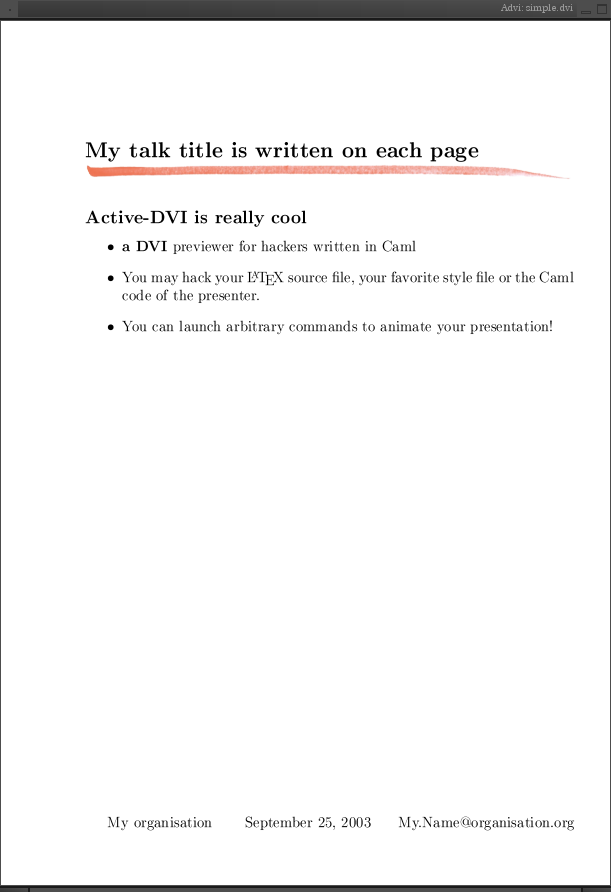
\includegraphics{simple.mps}
\end{minipage}
\begin{minipage}{0.8\linewidth}
\small\begin{ocaml}
[ Box.draw (Box.tex "\\LaTeX");
  Box.draw (Box.shift (Point.pt (cm 1., zero)) 
	     (circle (empty ()))) ]
\end{ocaml}
\end{minipage}

\medskip\noindent
Une figure \mlpost\ est simplement une liste de commandes de
dessin. Ci-dessus, elle est réduite à deux occurrences de
\texttt{Box.draw}, la commande qui dessine une boîte.
% Notez que par défaut, le contour de la boîte contenant du \LaTeX n'a
% pas été tracé, alors que celui de la boîte vide a été tracé.

\paragraph{Placement relatif.}
Un principe que nous avons suivi lors de la conception de \mlpost{}
est de favoriser un placement relatif des objets plutôt qu'absolu.
Ceci permet d'obtenir des figures plus robustes. En effet, imaginons
que l'on veuille placer une boîte $A$ à \emph{droite} d'une boîte $B$.
Une première possibilité serait de spécifier les positions
approximativement, par exemple en donnant les abscisses 0 cm pour $A$
et 2 cm pour $B$. Cependant, si on change d'avis sur le contenu de
$A$ et que la taille de cette boîte change, $A$ risque alors de se
superposer à $B$. Il faut alors replacer toutes les boîtes de la
figure manuellement. Pour éviter ça, \mlpost\ propose diverses
méthodes pour placer les boîtes \emph{les unes par rapport aux
  autres}. On gagne alors du temps lors de la création et lors des
modifications de la figure.  L'exemple suivant utilise l'alignement
horizontal \verb|hbox|, où l'argument optionnel \texttt{padding}
permet de spécifier l'espacement horizontal entre deux boîtes :

\medskip
\begin{minipage}{0.2\linewidth}
  \includegraphics{align.mps}
\end{minipage}
\begin{minipage}{0.8\linewidth}
\small\begin{ocaml}
[ Box.draw (Box.hbox ~padding:(cm 1.) 
              [Box.tex "\\LaTeX"; 
               circle (empty ())]) ]
\end{ocaml}
\end{minipage}

\medskip\noindent Nous revenons plus en détail sur les boîtes et leur
implémentation dans la section~\ref{subsec:boxes}.

\paragraph{Persistance.}
Un autre choix que nous avons fait est celui de la
persistance~\cite{persistance} : 
lorsqu'un attribut d'une boîte (positionnement, couleur, etc.) est
modifié, on obtient une nouvelle boîte, identique à la première sauf
en l'attribut changé. En faisant le choix de structures de données
persistantes, nous permettons à l'ancienne boîte, avec ses attributs
inchangés, d'être préservée et encore accessible. Ainsi, on peut
réutiliser plus facilement une boîte à plusieurs endroits
du dessin, avec des attributs différents. Dans l'exemple suivant, on a
utilisé trois instances de la même boîte \texttt{b}, dont le contour
est tracé pour la deuxième.

\medskip
\begin{minipage}{0.22\linewidth}
  \includegraphics{persistance.mps}
\end{minipage}
\begin{minipage}{0.78\linewidth}
\small\begin{ocaml}
let b = 
  Box.hbox ~padding:(cm 1.) 
    [Box.tex "\\LaTeX"; circle (empty ())] 
in
[ Box.draw (Box.vbox 
    [b; set_stroke Color.black b; b]) ]
\end{ocaml}
\end{minipage}

%TODO exemple ici qui introduit les noms des boites et les avantages /
%inconvénients de la persistance

\subsection{Exemples}

Dans cette section, nous montrons quelques applications immédiates des
boîtes de \mlpost. 

% blocs mémoire (listes, etc.) -- JCF
% introduire Box.vblock
% introduire les noms de boites
\paragraph{Représentation de la mémoire.}
Un besoin récurrent lorsque l'on enseigne l'algorithmique ou les
concepts liés à un langage de programmation consiste à illustrer
la structure des données en mémoire par des schémas de la forme
\begin{center}
  \includegraphics{list123.mps}
\end{center}
Deux éléments sont nécessaires : le dessin des blocs d'une part et le
dessin des pointeurs d'autre part. Pour réaliser les blocs, on utilise
la fonction \texttt{Box.hblock} qui aligne des boîtes horizontalement,
leur donne une hauteur commune et trace leur contour. Voici un exemple
:

\medskip
\begin{minipage}{0.15\linewidth}
  \includegraphics{simple_block.mps}
\end{minipage}
\begin{minipage}{0.8\linewidth}
\small\begin{ocaml}
let b = Box.hblock ~pos:`Bot 
  [Box.tex "a"; Box.tex "b"; Box.tex "C"] in
[ Box.draw b ]
\end{ocaml}
\end{minipage}

\medskip\noindent À l'aide de \texttt{Box.hblock}, on peut facilement
écrire une fonction \texttt{cons} qui construit un bloc de taille 2,
dont le premier élément contient un texte \LaTeX\ arbitraire
\texttt{hd} et le second est soit vide, soit le symbole $\bot$, selon
la valeur du booléen \texttt{tl} :
\begin{ocaml}
let cons hd tl =
  let p1 = Box.tex ~name:"hd" hd in
  let p2 = Box.tex ~name:"tl" 
     (if tl then "" else "\\ensuremath{\\bot}") in
  Box.hblock [p1; p2]
\end{ocaml}
L'argument optionnel \texttt{\~{}name} permet de nommer les
sous-boîtes, de manière à pouvoir y accéder facilement par la suite.

Écrivons maintenant une fonction \texttt{pointer\_arrow} pour
matérialiser les pointeurs. Il s'agit de tracer une flèche entre deux
boîtes données \texttt{a} et \texttt{b}. Pour cela, on commence par
construire un chemin \texttt{p} reliant les centres de \texttt{a} et
\texttt{b}, que l'on tronque à l'endroit où il intersecte le bord de la boîte
\texttt{b} (avec la fonction \texttt{Path.cut\_after}). Puis on trace
l'origine de la flèche à l'aide d'un chemin réduit à un point (le
centre de \texttt{a}) et la flèche proprement dite à l'aide du chemin
\texttt{p}.

\medskip
\begin{minipage}{0.2\linewidth}
  \includegraphics{block_arrow.mps}
\end{minipage}
\begin{minipage}{0.8\linewidth}
\small\begin{ocaml}
let pointer_arrow a b =
  let p = pathp [Box.ctr a; Box.ctr b] in
  let p = Path.cut_after (Box.bpath b) p in
  let pen = Pen.scale (bp 4.) Pen.circle in
  Command.draw ~pen (pathp [Box.ctr a]) ++ 
  draw_arrow p
\end{ocaml}
\end{minipage}
%XXX virer ++ ?

\medskip\noindent On utilise ici le symbole infixe \texttt{++} qui
permet de concaténer des commandes de dessin. On utilise d'autre
part \texttt{bp}, qui est une unité propre à \metapost, proche du
point \postscript.

Nous avons maintenant tous les éléments nécessaires pour écrire une
fonction \texttt{draw\_list} qui prend en argument une liste \ocaml\
de fragments \LaTeX\ et réalise l'illustration correspondante. On
commence par construire les différents blocs constituant la liste :
\begin{ocaml}
let draw_list l =
  let rec make = function
    | [] -> []
    | [x] -> [cons x false]
    | x :: l -> cons x true :: make l in
\end{ocaml}
Puis on aligne ces blocs avec \texttt{Box.hbox}, en insérant de
l'espace horizontal avec l'option \texttt{padding} :
\begin{ocaml}
  let l = hbox ~padding:(bp 30.) (make l) in
\end{ocaml}
Pour dessiner les pointeurs, il suffit de parcourir la liste des
boîtes (qui ont été placées) et d'utiliser la fonction
\texttt{pointer\_arrow} précédente sur chaque paire de boîtes
consécutives :
\begin{ocaml}
  let rec arrows = function
    | [] | [_] -> nop
    | b1 :: (b2 :: _ as l) -> 
       pointer_arrow (Box.get "tl" b1) (Box.get "hd" b2) 
       ++ arrows l 
  in
\end{ocaml}
On utilise ici la fonction \texttt{Box.get} qui permet de récupérer
une sous-boîte par son nom. On accède ainsi aux boîtes nommées
respectivement \verb!"hd"! et \verb!"tl"! qui ont été créées par la
fonction \texttt{cons} puis encapsulées dans d'autres boîtes par les
fonctions d'alignement.
Enfin, on dessine les boîtes avec \texttt{Box.draw}, puis les flèches
avec la fonction \texttt{arrows} :
\begin{ocaml}
  [ Box.draw l; arrows (Array.to_list (Box.elts l)) ]
\end{ocaml}
On peut tester avec
\begin{ocaml}
  draw_list 
    (List.map (fun n -> Printf.sprintf "$\\sqrt{%d}$" n) 
    [1;2;3;4])
\end{ocaml}
qui donne bien le résultat attendu :
\begin{center}
  \includegraphics{another_list.mps}
\end{center}

% De manière générale, les
% fonctions \texttt{Box.tex} et \texttt{Box.box}, ainsi que toutes les
% autres fonctions de création de boîtes, disposent d'arguments
% optionnels \texttt{dx} et \texttt{dy} permettant de spécifier les
% marges séparant le contenu du contour de la boîte. 

\paragraph{Diagrammes de classes.}
Avec la fonction \texttt{Box.vblock}, analogue pour l'alignement
vertical de la fonction
\texttt{Box.hblock} introduite ci-dessus, il est facile
de dessiner des diagrammes UML. Supposons que l'on veuille dessiner
des schémas de classes tels que :
\begin{center}
  \includegraphics{uml_client.mps}
\end{center}
Pour cela, introduisons une fonction \texttt{classblock} qui attend le
nom de la classe ainsi que la liste des attributs et des méthodes. 
\begin{ocaml}
let classblock name attr_list method_list = 
  let vbox = Box.vbox ~pos:`Left in
  Box.vblock ~pos:`Left ~name
  [ tex ("{\\bf " ^ name ^ "}");
    vbox (List.map tex attr_list); 
    vbox (List.map tex method_list) ]
\end{ocaml}
Ici, le nom \texttt{name} de la classe est utilisé à la fois pour
désigner le schéma dans le diagramme (l'argument labelisé \url{~name}
de \texttt{Box.vblock}) et comme titre du schéma créé. Les attributs
et les méthodes sont alignés verticalement indépendamment, puis on
aligne le titre et les deux nouvelles boîtes obtenues en les
encadrant\footnote{Notez qu'au contraire de {\tt hbox} et {\tt vbox}, les
fonctions {\tt hblock} et {\tt vblock} tracent par défaut le contour
de leurs sous-boîtes.}.  On peut maintenant s'en servir pour dessiner un
petit diagramme de classes :

\medskip
\begin{minipage}{0.38\linewidth}
  \includegraphics[width=0.9\linewidth]{uml.mps}
\end{minipage}
\begin{minipage}{0.6\linewidth}
\small\begin{ocaml}
let a = classblock "BankAccount" 
  [ "balance : Dollars = $0$"] 
  [ "deposit ..."; ... ] in
let b = classblock "Client" 
  [ "name : String"; ...] [] in
let diag = 
  Box.vbox ~padding:(cm 1.) [a;b] 
in
[ Box.draw diag; 
  box_label_arrow ~pos:`Left 
    (Picture.tex "owns") 
    (get "Client" diag) 
    (get "BankAccount" diag) ]
\end{ocaml}
\end{minipage}
\vspace{1em}

Ici, on a d'abord créé deux schémas de classe avec la fonction
\texttt{classblock}. Ces schémas sont ensuite alignés verticalement,
et une flèche avec une étiquette est dessinée entre ces deux classes
avec \texttt{box\_label\_arrow}. Le code pour cette figure est
conceptuellement très simple, ne contient aucun placement absolu et ne
dépasse pas les 15 lignes de code.

% automate -- RB
\paragraph{Automates.}\label{sec:automates}
La théorie des langages est un domaine où l'on a  rapidement besoin de
dessiner des automates. Illustrons une façon 
d'utiliser \mlpost\ dans ce but. Nous allons définir les fonctions 
suivantes :
\begin{itemize}
\item \texttt{state} pour créer un état ;
\item \texttt{final} pour transformer un état en un état final ;
\item \texttt{initial} pour dessiner une flèche entrante sur un état initial ;
\item \texttt{transition} pour dessiner une transition d'un état à un autre ;
\item \texttt{loop} pour dessiner une transition d'un état vers lui-même.
\end{itemize}
On choisit de représenter les états par des boîtes \mlpost.  La
fonction \texttt{state} est juste une spé\-ci\-ali\-sa\-tion de la
fonction {\tt Box.tex} à un contour circulaire, définie par
l'application partielle suivante:
\begin{ocaml}
let state = Box.tex ~style:Circle 
                    ~stroke:(Some Color.black)
\end{ocaml}
Le paramètre \texttt{stroke} permet de spécifier si le contour doit
être tracé et, le cas échéant, dans quelle couleur. De manière
similaire, la fonction \texttt{final} est une spécialisation de la
fonction {\tt Box.box} dont le rôle consiste à rajouter un cercle
autour d'une boîte :
\begin{ocaml}
let final = Box.box ~style:Circle
\end{ocaml}

On peut déjà placer des états, finaux ou non,
et  les  dessiner.   Pour  le  placement,  on  utilise  les  fonctions
d'alignement    horizontal    et    vertical   \texttt{Box.hbox}    et
\texttt{Box.vbox}. On  suit donc le  principe consistant à  placer les
objets de façon relative, les uns par rapport aux autres.

\begin{minipage}{0.2\linewidth}
  \includegraphics{automate_1.mps}
\end{minipage}
\begin{minipage}{0.7\linewidth}
\begin{ocaml}
let states = Box.vbox ~padding:(cm 0.8)
  [ Box.hbox ~padding:(cm 1.4)
      [ state ~name:"alpha" "$\\alpha$";
        state ~name:"beta" "$\\beta$" ];
    final ~name:"gamma" 
      (state "$\\gamma$") ] in
[ Box.draw states ]
\end{ocaml}
\end{minipage}

\medskip\noindent On note que l'ensemble des états est lui-même une boîte,
\texttt{states}, contenant les états comme autant de sous-boîtes nommées.

La  fonction \texttt{initial} appose une  flèche entrante  à un
état.  Il  s'agit donc  d'une fonction  qui prend le nom d'un état
\texttt{q}  et qui 
renvoie une commande dessinant une  flèche vers \texttt{q}. On pourrait aussi
renvoyer une  boîte sans  contour contenant \texttt{q}  et la flèche,  ce qui
permettrait   d'utiliser  \texttt{initial}  de   la  même   façon  que
\texttt{final}.   Cependant, la  boîte  obtenue n'aurait  pas la  même
taille et  la même forme que  \texttt{q}, ce qui poserait  des problèmes pour
placer \texttt{q} ou pour dessiner des transitions vers ou à partir de
\texttt{q}. 
\begin{ocaml}
let initial (states : Box.t) name : Command.t =
  let q = Box.get name states in
  let p = Box.west q in
  Arrow.draw (Path.pathp 
    [Point.shift p (Point.pt (cm (-0.3), zero)); p])
\end{ocaml}
La fonction  accède à  la boîte \texttt{q}  par son  nom \texttt{name}
dans la  boîte \texttt{states} et détermine le point d'arrivée de la
flèche avec \texttt{Box.west}. On pourrait généraliser cette fonction
pour spécifier la position de la flèche.

La fonction \texttt{transition} dessine une flèche d'un état à un
autre. Cette fonction prend deux arguments optionnels \texttt{outd} et
\texttt{ind} pour spécifier, en degrés, la direction sortante et la
direction entrante de la flèche. On doit les convertir en vecteurs
directeurs pour les passer\footnote{Nous utilisons ici une
  fonctionnalité d'\ocaml{} qui permet d'accéder à des arguments
  optionnels sans spécifier leur valeur par défaut, sous la forme d'un
  type {\tt option}. Nous passons ensuite directement ces valeurs de
  type {\tt option}, en tant qu'arguments optionnels, à la fonction
  {\tt cpath} par la syntaxe {\tt cpath ?outd ?ind x y}.} à \texttt{cpath}, qui
calcule un chemin allant du bord d'une boîte au bord d'une autre
boîte. Ce chemin est ensuite donné à la fonction \texttt{Arrow.draw}
qui trace la flèche en plaçant une étiquette \texttt{tex} à la
position \texttt{pos}.
\begin{ocaml}
let transition states tex pos ?outd ?ind x_name y_name = 
  let x = Box.get x_name states 
  and y = Box.get y_name states in
  let outd = match outd with 
    | None -> None | Some a -> Some (vec (dir a)) in
  let ind = match ind with 
    | None -> None | Some a -> Some (vec (dir a)) in
  Arrow.draw ~tex ~pos (cpath ?outd ?ind x y) 
\end{ocaml}

La fonction \texttt{loop} est similaire à la fonction
\texttt{transition}, mais elle doit calculer un chemin plus complexe.
En effet, \texttt{cpath} appliqué à deux boîtes identiques renvoie un
chemin vide et on ne peut donc pas l'utiliser. À la place, on calcule
un point $A$ suffisamment éloigné de la boîte et on trace un chemin
qui part du centre, qui passe par $A$ puis qui revient au centre. On
utilise au passage la fonction \texttt{knotp} qui permet de spécifier
un point avec une tangente, et \texttt{pathk} qui transforme une liste 
de tels points en un chemin.

\begin{minipage}{0.3\linewidth}
  \includegraphics{loop_explain.mps}
\end{minipage}
\begin{minipage}{0.2\linewidth}
\small\begin{ocaml}
let loop states tex name =
  let box = Box.get name states in
  let a = Point.shift (Box.south box) 
    (Point.pt (cm 0., cm (-0.4))) in
  let c = Box.ctr box in
  let p = Path.pathk [
    knotp ~r:(vec (dir 225.)) c;
    knotp a;
    knotp ~l:(vec (dir 135.)) c;
  ] in
  let bp = Box.bpath box in
  Arrow.draw ~tex ~pos:`Bot 
    (cut_after bp (cut_before bp p))
\end{ocaml}
\end{minipage}

Ici encore, on pourrait généraliser cette fonction
pour spécifier la position de la flèche.
On  peut maintenant  dessiner  facilement des  automates en  utilisant
cette bibliothèque.

\medskip
\begin{minipage}{0.2\linewidth}
  \includegraphics{automate.mps}
\end{minipage}
\begin{minipage}{0.2\linewidth}
\small\begin{ocaml}
let automate =
  let states = ... in
  [ Box.draw states;
    transition states "a" `Lowleft 
      "alpha" "gamma";
    transition states "b" `Lowright 
      "gamma" "beta";
    transition states "c" `Top ~outd:25. 
      ~ind:335. "alpha" "beta";
    transition states "d" `Bot ~outd:205. 
      ~ind:155. "beta" "alpha";
    loop states "e" "gamma"; 
    initial states "alpha" ]
\end{ocaml}
\end{minipage}


\subsection{Exemples utilisant des calculs en \ocaml}

Cette section illustre l'un des avantages de \mlpost: la capacité de
dessiner directement un objet que l'on a calculé/programmé en \ocaml.

% plot -- SL
\paragraph{Graphe de fonction.}
Un exemple simple de dessin résultant d'un calcul est celui du graphe
d'une fonction.  \mlpost\ fournit un module \texttt{Plot} à cet effet.
La figure suivante montre un exemple basique
d'utilisation de cette extension :

\medskip
\begin{minipage}{0.28\linewidth}
  \includegraphics[width=0.9\linewidth]{graph_sqrt.mps}
\end{minipage}
\begin{minipage}{0.65\linewidth}
\small\begin{ocaml}
let u = cm 1. in
let sk = Plot.mk_skeleton 4 3 u u in
let label = Picture.tex "$y=...$", 
            `Upleft, 3 in
let f x = sqrt (float x +. 0.5) in
[ Plot.draw_func ~label f sk; 
  Plot.draw_simple_axes "$x$" "$y$" sk ]
\end{ocaml}
\end{minipage}

\medskip\noindent La fonction \texttt{mk\_skeleton} permet de construire un
cannevas de 4 unités sur 3, qui est l'objet de base de l'extension
\texttt{Plot}. Il est alors possible de dessiner un graphe de fonction
et des axes au sein de ce cannevas, comme illustré ci-dessus.
L'extension dispose de beaucoup d'options (tracé de la grille,
affichage des abscisses et ordonnées, différents types de graphes de
fonctions) qui permettent de réaliser des figures plus complexes,
telle que celle décrite dans le paragraphe suivant.

\paragraph{Abstractions d'horloges dans un système synchrone flot-de-données.}
L'exemple ci-dessous, réalisé par Florence Plateau, 
provient d'un problème réel~\cite{MandelPlateau08} et illustre un
certain nombre des possibilités de l'extension \texttt{Plot}.
%
%
Ainsi les fonctions illustrées sur cette figure ont été codées comme des
fonctions \ocaml{} standard. De plus, la ligne intermédiaire dans la
partie située sous le graphe principal, et dénotée par $w_2$,
représente les discontinuités de la fonction $f_{w_2}$ du graphe
principal. Cette ligne est calculée \textit{directement} à partir de
la fonction $f_{w_2}$ ; si l'on décide de changer la fonction
$f_{w_2}$, la ligne $w_2$ sera mise à jour automatiquement. Cela est
également vrai pour certaines étiquettes de la figure, comme l'abscisse
$[w_2]_5$. Ceci offre une flexiblité très intéressante lors de la
phase de développement d'une telle figure.

\begin{figure}[h]
  \centering
  \begin{center}
    \medskip
    \includegraphics{florence.mps}
  \end{center}
  %\caption{expliquer de quoi ça parle}
  \label{fig:florence}
\end{figure}

\paragraph{Bresenham.}
À titre de dernier exemple, supposons que l'on veuille illustrer
l'algorithme de tracé de segment de Bresenham~\cite{bresenham}, par
exemple sur le segment reliant le point $(x_1,y_1)=(0,0)$ au point
$(x_2,y_2)=(9,6)$. Pour cela, on commence par stocker le résultat de
l'algorithme dans un tableau \texttt{bresenham\_data}, tel que
$\texttt{bresenham\_data.(}x\texttt{)}$ donne l'ordonnée du point
d'abscisse $x$. 
\begin{ocaml}
let x2 = 9 and y2 = 6
let bresenham_data = Array.create (x2+1) 0 
let () = (* remplissage du tableau a *)
         (* avec l'algorithme de Bresenham *) ...
\end{ocaml}
On peut alors réaliser la figure très facilement, à l'aide de la
fonction \texttt{Box.gridi} fournie par \mlpost, qui construit une
matrice de boîtes alignées à partir d'une largeur, d'une hauteur et
d'une fonction construisant la boîte $(i,j)$,
d'une manière analogue à \texttt{Array.create\_matrix}.

\medskip
\begin{minipage}{0.32\linewidth}
  \includegraphics{bresenham0.mps}
\end{minipage}
\begin{minipage}{0.7\linewidth}
\vspace*{0.8em}
\small\begin{ocaml}
let width = bp 6. 
and height = bp 6. in
let g = Box.gridi (x2+1) (y2+1) 
  (fun i j -> 
    let fill = 
      if bresenham_data.(i) = y2 - j 
      then Some Color.red else None in
    Box.rect ?fill 
      (Box.empty ~width ~height ())) 
in
[ Box.draw g ]
\end{ocaml}
\end{minipage}

\medskip\noindent Les boîtes sont des boîtes vides de 6 points de
côté, créées avec \texttt{Box.empty}. Pour les boîtes correspondant à
des points dessinés par l'algorithme de Bresenham, on indique que la
boîte doit être remplie en rouge, à l'aide de l'argument optionnel
\texttt{fill}. 

Pour parachever la figure, on va ajouter des étiquettes indiquant les
coordonnées des deux extrémités du segment. Pour placer une étiquette
à côté de la case $(i,j)$, on récupère la boîte correspondante à
l'aide de \texttt{Box.nth}, puis on récupère un point particulier de
cette boîte (par exemple le point au milieu en bas avec
\texttt{Box.south}), puis enfin on trace l'étiquette avec
\texttt{Command.label}.

\medskip
\begin{minipage}{0.28\linewidth}
\vspace*{0.8em}
\hspace*{-1.4em}\includegraphics{bresenham.mps}
\end{minipage}
\begin{minipage}{0.7\linewidth}\small
\begin{ocaml}
let bresenham = 
  let width = bp 6. 
  and height = bp 6. in
  let g = ... in
  let get i j = 
    Box.nth i (Box.nth (y2-j) g) in
  let label pos s point i j =
    Command.label ~pos (Picture.tex s) 
      (point (get i j)) in
  [ Box.draw g;
    label `Bot "0" Box.south 0 0; 
    label `Bot "$x_2$" Box.south x2 0;
    label `Left "0" Box.west 0 0; 
    label `Left "$y_2$" Box.west 0 y2 ]
\end{ocaml}
\end{minipage}

\section{Architecture logicielle}\label{archi}

La figure~\ref{fig:etapes} montre le fonctionnement de \mlpost.  Tout
d'abord, \mlpost\ est un outil de génération de fichier \metapost\
sous forme de bibliothèque \ocaml. À l'aide de cette bibliothèque,
l'utilisateur écrit un programme qui, à l'exécution, construit un
arbre de syntaxe abstraite \metapost. Cet arbre est imprimé dans un
fichier \verb|figure.mp| qui est lu par \metapost\ pour générer un ou
plusieurs fichiers \postscript\footnote{Ces fichiers n'ont pas le
  suffixe \texttt{.ps} car il leur manque l'en-tête.}. L'inclusion de
ces figures dans un document \LaTeX{} se fait simplement en utilisant
la commande \verb|\includegraphics| du package \textsf{graphicx}. Pour
compiler le document \LaTeX{} avec {\tt pdflatex}, il suffit de
changer l'extension des figures générées, ce qu'une option de l'outil
\mlpost{} permet de faire facilement.

\begin{figure}[h]
\begin{center}
\includegraphics[width=\textwidth]{stages.mps}
\end{center}
  \caption{Architecture de \mlpost}\label{fig:etapes}
\end{figure}

Il est important de noter que le fichier \metapost\ de sortie n'est
pas obtenu par {\em compilation} du code source \ocaml, mais
par une \emph{exécution} du programme qui construit un arbre de syntaxe
abstraite \metapost. Cette méthode a l'inconvénient qu'une boucle ou
itération dans le programme de départ sera traduite par une suite de
commandes obtenues par le déroulement de la boucle, et non par une
construction de boucle du langage cible. Ceci étant dit, dans notre
cas, le coût supplémentaire est faible, puisque \metapost\ déroule
également les boucles dans les fichiers \postscript\ de sortie.

% schéma de l'architecture
\begin{figure}[ht]
  \begin{center}
    ~\\[0.5em]
    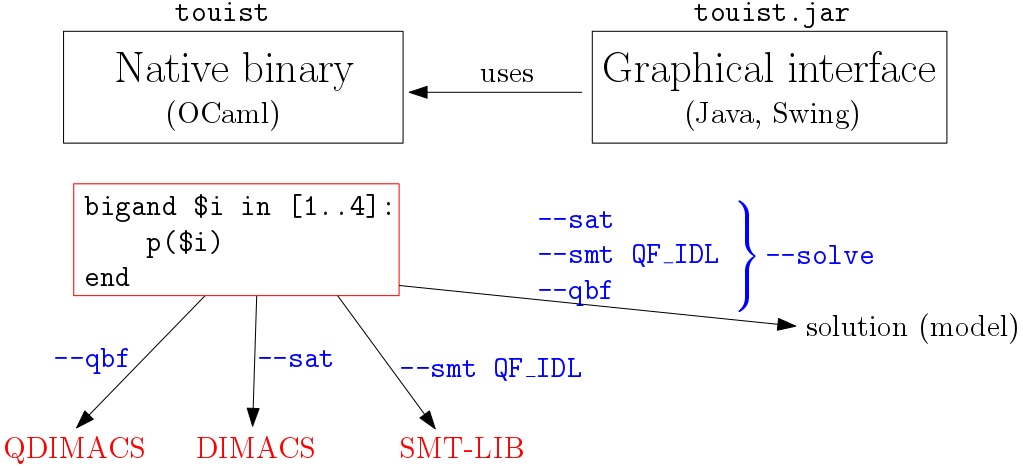
\includegraphics{architecture.mps} 
  \end{center}
  \vspace*{-1em}
  \caption{Architecture de \mlpost}\label{fig:archi}
\end{figure}

L'architecture générale de \mlpost{} est schématisée en
figure~\ref{fig:archi}. Au niveau le plus bas se trouvent les interfaces
correspondant aux types primitifs de \metapost. Ce sont ces objets qui sont
{\it in fine} traduits en du code \metapost, et nous les décrivons de manière
plus détaillée dans la section~\ref{subsec:types}. La couche intermédiaire
contient des éléments que nous estimons être de bas niveau mais qui ne sont
pas présents dans \metapost : ils sont propres à \mlpost\ et ont été
construits à partir de la couche inférieure. Les sections~\ref{subsec:boxes}
et \ref{subsec:arrows} reviennent plus en détail sur deux de ces modules,
respectivement \texttt{Box} et \texttt{Arrow}.
Enfin, on trouve au plus haut niveau des modules tels que
le module \texttt{Plot} présenté dans la section précédente.
L'intégralité des modules de \mlpost\ est empaquetée dans un module
\texttt{Mlpost}, afin de ne pas polluer l'espace de noms d'\ocaml.

\subsection{Types primitifs de \metapost}\label{subsec:types}

La couche de bas niveau de \mlpost\ est une interface fidèle à \metapost. Elle
comporte tous les types de base de \metapost~:

\begin{description}

  \item[Le type numérique (module \texttt{Num})] représente des longueurs.
    En première approximation, ce type pourrait être assimilé au type
    \texttt{float} d'\ocaml, 
    mais certaines valeurs, telle que  la taille d'un élément \LaTeX, ne sont
    connues qu'à l'interprétation du fichier \metapost.  La plupart des
    calculs sont donc effectués de 
    manière symbolique et le type \texttt{Num.t} doit donc être abstrait.

  \item[Le type point (module \texttt{Point})] représente des points
    dans l'espace à deux dimensions. Pour les mêmes raisons que les
    numériques, les points ne sont pas simplement des paires de flottants, mais
    doivent être représentés de manière symbolique. Le type
    \texttt{Point.t} est également utilisé pour représenter les vecteurs.

  \item[Les chemins (module \texttt{Path})] sont des lignes représentées par
    des courbes de Bézier. Ils sont à la base de tout dessin \metapost. Toutes
    les possibilités de construction de chemin dans \metapost\ ont été
    interfacées. On peut dessiner des lignes droites ou des lignes courbes en
    précisant les points de contrôle, la tension de la courbe, etc.
    
  \item[Les transformations (module \texttt{Transform})] permettent
    d'appliquer une transformation linéaire à un objet quelconque. Il est
    ainsi possible de déplacer des objets, les redimensionner,
    les faire pivoter ou encore combiner toutes ces transformations.

  \item[Les plumes (module \texttt{Pen})] permettent de choisir 
    l'épaisseur et la forme du stylo utilisé pour dessiner les
    chemins.

  \item[Les figures (module \texttt{Picture})] permettent de
    rassembler plusieurs éléments graphiques en un seul, qu'il
    s'agisse d'éléments \LaTeX\ ou de commandes de dessin arbitraires.
    Le type \texttt{Picture.t} permet de traiter
    une figure arbitrairement complexe comme un objet de base que l'on
    peut copier, transformer, etc.
    Le module \texttt{Picture} permet également de découper une figure
    à l'aide d'une surface décrite par un chemin clos
    (\textit{clipping}). 

\end{description}
Les autres types \metapost\ (chaînes de caractères, booléens, couleurs)
sont directement représentés en \ocaml. L'interface de \mlpost\ contient
aussi un module \texttt{Command} qui définit le type des commandes
\metapost : commandes de dessin, de remplissage, itérations,  séquences,
etc.

\paragraph{Dépendances circulaires.}
La réalisation de ces modules de bas niveau présente quelques
difficultés. Premièrement, la plupart des modules présentés sont {\em
  a priori} mutuellement récursifs : par exemple, les transformations
s'appliquent à tous les autres objets, donc chaque module contient une
fonction
\begin{ocaml}
  val transform : Transform.t -> t -> t
\end{ocaml}
où le type \texttt{t} représente le type principal du module en
question.  D'un autre côté, les transformations sont elles-mêmes
construites à l'aide de numériques et de points:
\begin{ocaml}
  val shifted : Point.t -> t
\end{ocaml}
où \texttt{t} est le type des transformations.  Des dépendances
circulaires existent aussi entre types et sont aggravées par la
représentation symbolique des objets (par exemple, les projections
\texttt{xpart} et \texttt{ypart} du module \texttt{Point} doivent
retourner des numériques et non des flottants).

Nous souhaitons réaliser ces différents modules dans des fichiers
différents mais \ocaml\ ne permet pas de dépendances
circulaires entre des fichiers. Notre solution consiste à définir tous
les \emph{types} dans un seul fichier \texttt{types.mli}.
Chaque module fait maintenant référence à ce fichier. Par exemple,
dans le fichier \texttt{path.ml}, qui fournit l'implémentation du
module \texttt{Path}, on trouvera
\begin{ocaml}
  type t = Types.path
\end{ocaml}
La dépendance circulaire entre les modules est ainsi cassée de manière très
classique. 
En revanche, on souhaite cacher l'existence du module \texttt{Types} 
pour les deux raisons suivantes : 
\begin{itemize}
\item la clarté des messages d'erreur ;
\item la clarté de la documentation générée par \texttt{ocamldoc}.
\end{itemize}
On souhaite donc rétablir la circularité entre les modules
au sein de l'interface du module \texttt{Mlpost}.
Pour cela, on écrit un unique fichier
\texttt{mlpost.mli} qui contient les définitions des signatures des
modules à exporter :

\medskip
\begin{minipage}{0.3\textwidth}
\small\begin{ocaml}
module rec Point : sig
  type t
  val xpart : t -> Num.t
  ...
end
and Num : sig
  type t
  ...
end
and Path : sig
  type t
  ...
end
...
\end{ocaml}
\end{minipage}
\begin{minipage}{0.6\textwidth}
  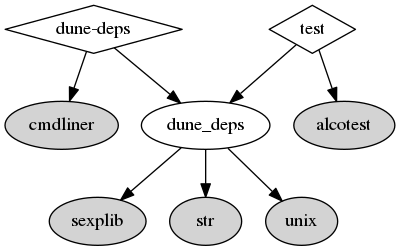
\includegraphics[width=1\textwidth]{deps.mps}
\end{minipage}

Toutes ces signatures sont déclarées de manière mutuellement
récursive. La signature de \texttt{Point} peut ainsi faire référence à
\texttt{Path} et inversement.  On notera que les types tels que
\texttt{Point.t} sont maintenant abstraits dans l'interface, rendant
invisible l'existence du module \texttt{Types}.  Par ailleurs, les
implémentations de ces modules sont contenues dans des fichiers
indépendants \texttt{num.ml}, \texttt{point.ml}, etc., qui sont
compilés avec l'option {\tt -for-pack Mlpost}.  Cet agencement est en
outre très pratique pour la documentation de l'API : c'est uniquement
le fichier \texttt{mlpost.mli} qui sert d'entrée à l'outil
\texttt{ocamldoc}.

\paragraph{Hash-consing et traduction vers \metapost.}

Le choix d'une représentation symbolique de la plupart des objets impose
des efforts supplémentaires pour minimiser l'utilisation de la mémoire
et la taille des fichiers \metapost\ de sortie. En effet, l'arbre de
syntaxe abstraite (AST) contient beaucoup de n\oe uds identiques mais
construits de manière différente, qui prennent donc inutilement de la
place aussi bien en mémoire que dans le fichier \metapost\ généré. C'est
d'autant plus gênant que \metapost\ devra lire ce fichier et passera
donc davantage de temps sur des calculs répétés.

Pour y remédier, nous utilisons la technique du {\em
hash-consing}~\cite{ConchonFilliatre06wml} appliquée à l'arbre de syntaxe
abstraite. Cette technique permet de partager des valeurs structurellement
égales. Elle utilise une table de hachage globale qui stocke toutes les valeurs
déjà créées. Avant de créer un nouvel objet, on regarde dans cette table si un
objet structurellement égal existe déjà. Pour que le calcul de la valeur de
hachage soit efficace, chaque (sous-)terme
vient avec sa valeur de hachage. Le partage réalisé est maximal, ce
qui permet de substituer l'égalité physique (\texttt{==}) à l'égalité
structurelle (\texttt{=}). 

Cette technique diminue l'utilisation de la mémoire, mais ne change rien {\em a
priori} à la taille des fichiers générés. La structure hash-consée {\em
réalise} le partage, mais elle ne sait pas quels sont les n\oe uds
effectivement 
utilisés au moins deux fois. Pour cela, on réalise un simple parcours
en profondeur de la structure, en comptant les occurrences de chaque
n\oe ud.  Il est néanmoins
possible de rencontrer une nouvelle fois un sous-n\oe ud d'une structure,
comme le montre l'exemple ci-dessous :

\begin{center}
\includegraphics[scale=1.5]{sharing.mps}
\end{center}

\noindent Dans cette configuration, le n\oe ud $f$ est réellement utilisé deux
fois, alors que le n\oe ud $e$ n'est utilisé qu'une seule fois, par le
n\oe ud $d$, même si celui-ci est utilisé deux fois à son tour.
Autrement dit, on comptabilise pour chaque n\oe ud le nombre de
flèches incidentes.

Après cette analyse, la génération du fichier \metapost\ devient très simple :
il suffit de traverser de nouveau l'arbre de syntaxe abstraite et,
quand on visite un n\oe ud 
qui est utilisé au moins deux fois,  on construit une définition
\metapost\ pour cet objet. Il faut néanmoins
prendre en compte les particularités syntaxiques de \metapost\ telles que la
précédence inhabituelle des opérateurs arithmétiques et la restriction de
l'application de certaines constructions à des variables. De cette façon, on
arrive à avoir du code \metapost\ relativement petit\footnote{En l'absence de
boucles \texttt{for} et de macros dans le code \metapost, nous avons observé,
sans avoir fait de tests très exhaustifs, une taille du code généré du
même ordre de grandeur que celle du code \metapost\ écrit à la main.},
malgré la délégation des calculs à \metapost. 

\subsection{Boîtes}\label{subsec:boxes}

Comme nous l'avons illustré déjà maintes fois, les boîtes de \mlpost\
peuvent être réduites à de simples objets \LaTeX\ ou bien être
constituées d'un ensemble d'autres boîtes. Le type des boîtes est donc
un type récursif de la forme suivante :
\begin{ocaml}
type t =
  { name : string option;
    width : Num.t;  height : Num.t; 
    pen : Pen.t option; ...
    desc : desc; }
    
and desc = 
  | Emp
  | Pic of Picture.t
  | Grp of t array * t Smap.t
\end{ocaml}
Chaque boîte est éventuellement nommée (champ \texttt{name}), possède
un certain nombre d'attributs (position, taille, couleur, bordure,
remplissage, etc.) et sa nature est donnée par le champ \texttt{desc}.
Ce dernier indique s'il s'agit d'une boîte vide, d'une image ou bien
d'une boîte composite. Dans ce dernier cas, les sous-boîtes sont
contenues dans un tableau, qui est accompagné d'une table (réalisée
par le module \texttt{Smap}) permettant un accès plus rapide à une 
sous-boîte par son nom.

Le dessin d'une boîte est immédiat. On trace d'une part son contour et
d'autre part son contenu. Ce dernier est soit
une boîte atomique directement dessinée à l'aide de
\texttt{Command.draw\_pic}, soit une boîte composite dont le dessin
est tout simplement obtenu en dessinant récursivement chaque sous-boîte.

Pour réaliser les diverses fonctions de placement, on commence par
écrire une fonction de translation d'une boîte par un vecteur donné :
\begin{ocaml}
  Box.shift : Point.t -> Box.t -> Box.t
\end{ocaml}
Cette fonction est naturellement récursive sur la structure de la
boîte. Il est important de noter que cette fonction renvoie une
\emph{nouvelle} boîte, sans altérer son argument (les boîtes sont
persistantes). Une fois cette fonction donnée, il est aisé de réaliser
les fonctions \texttt{Box.hbox}, \texttt{Box.hblock}, etc.

\subsection{Flèches} \label{subsec:arrows} %% RB

\metapost\ ne propose qu'un seul type de flèche.
Une flèche \metapost\ suit  un chemin arbitraire   mais son tracé est
limité aux différents styles de trait (plume et pointillés) et la tête
de flèche est toujours la même : 
\begin{center}
\includegraphics[width=\textwidth]{arrow_metapost.mps}
\end{center}
Avec \mlpost, l'utilisateur peut créer ses propres catégories de
flèches à l'aide du module \texttt{Arrow}. Celui-ci propose deux types :
\begin{itemize}
\item  Le  type \texttt{head}  décrit  comment  dessiner  une tête  de
  flèche.   Les  éléments de  type  \texttt{head}  sont des  fonctions
  prenant en argument la position et la direction de la tête de flèche
  et renvoyant une commande dessinant la tête de flèche.
\item Le  type abstrait \texttt{kind} décrit une  catégorie de flèche.
  Une catégorie décrit les différents éléments dans le dessin d'une
  flèche, les têtes de flèche pouvant en réalité être placées
  n'importe où le long de la flèche.
  Pour construire une nouvelle catégorie, on  part de  la catégorie
  vide et on  ajoute des traits et des têtes.
\end{itemize}
La  fonction  \texttt{draw}  permet   de  dessiner  une  flèche  d'une
catégorie donnée  en suivant un  chemin donné. Les flèches  sont alors
dessinées  en   utilisant  les   primitives  de  \metapost.    Ceci  a
l'inconvénient  d'utiliser   plus  de  ressources   mais   permet
d'imaginer de nombreuses catégories de flèches.

On peut en particulier retrouver les flèches de \metapost. On part d'un
corps vide et on 
lui ajoute un trait normal sur  toute la longueur.  On ajoute enfin une tête
triangulaire remplie, et on obtient :

\medskip
\begin{minipage}{0.2\linewidth}
  \includegraphics{arrow_simple.mps}
\end{minipage}
\begin{minipage}{0.2\linewidth}
\begin{ocaml}
let kind =
  Arrow.add_head 
    ~head:Arrow.head_triangle_full
    (Arrow.add_line Arrow.empty) in 
[ Arrow.draw ~kind (...path...) ]
\end{ocaml}
\end{minipage}

\medskip
La  section~\ref{sec:automates}  contient   une  figure  décrivant  le
fonctionnement de la fonction \texttt{loop}. Pour les besoins de cette
figure, on  a créé un  type de flèche  spécial, composé d'un  début et
d'une fin en pointillés et avec une tête placée différemment :
\begin{center}
\includegraphics[width=\textwidth]{arrow_loop_explain.mps}
\end{center}
Le code permettant d'obtenir cette  catégorie de flèche est le suivant
:
{\small
\begin{ocaml}
let kind =
  Arrow.add_belt ~point:0.9
    (Arrow.add_line ~dashed:Dash.evenly ~to_point:0.1
       (Arrow.add_line ~dashed:Dash.evenly ~from_point:0.9
          (Arrow.add_line ~from_point:0.1 ~to_point:0.9
             Arrow.empty)))
\end{ocaml}
}

\section{Conclusion}\label{conclusion}

Nous avons présenté \mlpost, une bibliothèque \ocaml\ au dessus de
\metapost. Nous espérons avoir convaincu le lecteur des avantages que la
présentation sous forme de bibliothèque apporte : familiarité avec le
langage pour les programmeurs \ocaml, typage fort, des
constructions de programmation de haut niveau, des dessins résultants
de calculs arbitraires, etc.  
\mlpost\ fournit volontairement un nombre restreint de primitives, car
l'utilisateur peut aisément construire des
extensions au dessus de \mlpost. En cela, \mlpost\ diffère de
bibliothèques \LaTeX\ telles que \nomdetikz\ ou \pstricks, où de très
nombreuses fonctionnalités sont fournies mais où il est très difficile
d'en ajouter pour qui ne maîtrise pas \TeX.

L'une des forces de \mlpost\ est de proposer un style déclaratif, là
où la majorité des bibliothèques graphiques propose un style
impératif. Ceci permet en particulier un \emph{partage} immédiat de
sous-éléments dans une ou plusieurs figures.
Une autre force de \mlpost\ est le typage statique directement hérité
d'\ocaml. On évite ainsi l'immense majorité des erreurs à l'exécution
de \metapost, souvent cryptiques. Il reste néanmoins les erreurs
éventuellement contenues dans les extraits de \LaTeX\ ou les erreurs
de nature géométrique telles que le remplissage d'un chemin en forme
de 8. Nous pourrions envisager d'utiliser des types \ocaml\ plus
précis, par exemple pour distinguer les chemins clos et non clos ou
encore les points et les vecteurs.

Il reste une fonctionnalité intéressante de \metapost\ qui n'est pas
interfacée dans \mlpost~: la résolution d'équations linéaires.  Il y a
deux raisons à cela. D'une part, les équations servent souvent au
placement implicite, et \mlpost\ fournit une alternative sous la forme
de fonctions d'alignement de boîtes. D'autre part, la résolution
d'équations de \metapost\ procède de manière impérative et il n'est
pas simple de l'intégrer dans le contexte déclaratif qui est le nôtre.
Ceci étant dit, il serait intéressant d'explorer des méthodes de
placement plus automatiques que celles que nous proposons, par exemple
inspirées de la manière dont \TeX{} mets en page lignes, pages et
paragraphes.

Enfin, il est important de noter que \mlpost\ n'est pas lié à
\metapost\ de manière intrinsèque. On pourrait facilement ajouter une
sortie \nomdetikz, ou même directement une sortie \postscript\ à
condition d'utiliser une technique similaire à celle de \metapost\
pour l'inclusion de \LaTeX.

\medskip
\noindent
\vbox{
\begin{center}
  \includegraphics[width=0.3\textwidth]{ford.mps}

\medskip
\begin{minipage}{0.7\textwidth}
  \begin{center}
    \bf Remerciements
  \end{center}
  \centering Les auteurs tiennent à remercier Florence Plateau,
  Yannick Moy et Claude Marché pour leur contribution à \mlpost,
  Sylvie Boldo pour la suggestion du titre de l'article et les
  relecteurs pour leurs remarques.
\end{minipage}

\medskip
  \includegraphics[angle=180,width=0.3\textwidth]{ford.mps}
\end{center}
}

% La bibliographie
% N'oubliez pas de l'inclure lors de votre soumission.
\begin{thebibliography}{10}

\bibitem{haskell}
{Le langage Haskell}.
\newblock \url{http://www.haskell.org/}.

\bibitem{ocaml}
{Le langage Objective Caml}.
\newblock \url{http://caml.inria.fr/}.

\bibitem{bresenham}
Jack~E. Bresenham.
\newblock Algorithm for computer control of a digital plotter.
\newblock {\em IBM Systems Journal}, 4(1):25--30, January 1965.

\bibitem{mlpictex}
Emmanuel Chailloux and Asc\'ander Su\'arez.
\newblock {\mlpictex}, a picture environment for {\LaTeX}.
\newblock In {\em Workshop on {ML}}, pages 79--90, 1994.

\bibitem{MandelPlateau08}
Albert Cohen, Louis Mandel, Florence Plateau, and Marc Pouzet.
\newblock {Abstraction of Clocks in Synchronous Data-flow Systems}.
\newblock In {\em The Sixth ASIAN Symposium on Programming Languages and
  Systems (APLAS)}, Bangalore, India, December 2008.

\bibitem{ConchonFilliatre06wml}
Sylvain Conchon and Jean-Christophe Filli\^atre.
\newblock {Type-Safe Modular Hash-Consing}.
\newblock In {\em ACM SIGPLAN Workshop on ML}, Portland, Oregon, September
  2006.

\bibitem{persistance}
J.~R. Driscoll, N.~Sarnak, D.~D. Sleator, and R.~E. Tarjan.
\newblock {Making Data Structures Persistent}.
\newblock {\em Journal of Computer and System Sciences}, 38(1):86--124, 1989.

\bibitem{pstricks}
T.~Van~Zandt et~al.
\newblock {PSTricks}.
\newblock \url{http://tug.org/PSTricks/}.

\bibitem{fmpost}
Meik Hellmund, Ralf Hinze, Joachim Korittky, Marco Kuhlmann, Ferenc W\'agner,
  and Peter Simons.
\newblock {\fmpost}.
\newblock \url{http://cryp.to/funcmp/}.

\bibitem{metapost}
John Hobby.
\newblock \metapost, 1994.
\newblock \url{http://plan9.bell-labs.com/who/hobby/MetaPost.html}.

\bibitem{metafont}
Donald~E. Knuth.
\newblock {\em The {\metafont} Book}.
\newblock Addison-Wesley, 1984.

\bibitem{dia}
Alexander Larsson.
\newblock {Dia}.
\newblock \url{http://live.gnome.org/Dia}.

\bibitem{postscript}
Glenn~C. Reid.
\newblock {\em {PostScript Language Program Design}}.
\newblock Addison-Wesley Longman Publishing Co., Inc., Boston, MA, USA, 1988.

\bibitem{xfig}
Brian~V. Smith.
\newblock {Xfig}.
\newblock \url{http://www.xfig.org/}.

\bibitem{tikz}
Till Tantau.
\newblock {PGF and TikZ -- Graphic systems for \TeX}.
\newblock \url{http://sourceforge.net/projects/pgf/}.

\end{thebibliography}
%\bibliographystyle{plain}
%\bibliography{./biblio}

\vfill

%\pagebreak
%\thispagestyle{colloquetitle}
%\cleardoublepage
\end{document}

% Local Variables:
% coding: iso-latin-1
% ispell-local-dictionary: "francais"
% End:
